% ==============================================================
% CAPIM SOFTWARE — ANÁLISE DO SISTEMA DE GESTÃO DA INOVAÇÃO
% PRO3584 - Projeto, Processo e Gestão da Inovação
% Escola Politécnica da Universidade de São Paulo
% Departamento de Engenharia de Produção
% Professor: Mario Sergio Salerno
% Grupo 6
% ==============================================================

\documentclass[
    12pt, openright, twoside, a4paper,
    chapter=TITLE, section=TITLE,
    english, brazil
]{abntex2}

\usepackage[T1]{fontenc}
\usepackage[utf8]{inputenc}
\usepackage{lmodern}
\usepackage{microtype}
\usepackage{indentfirst}
\usepackage{graphicx}
\usepackage{booktabs}
\usepackage{tabularx}
\usepackage{longtable}
\usepackage{multirow}
\usepackage{float}
\usepackage{caption}
\usepackage{subcaption}
\usepackage{amsmath}
\usepackage{listings}
\usepackage{xcolor}
\usepackage{hyperref}
\usepackage{url}
\usepackage{setspace}
\usepackage{geometry}
\usepackage{csquotes}
\usepackage{tikz}
\usetikzlibrary{positioning, arrows.meta, shapes.geometric, fit, matrix}
\usepackage[style=abnt, backend=biber]{biblatex}

\geometry{top=3cm, bottom=2cm, left=3cm, right=2cm}
\raggedbottom

\addbibresource{referencias/referencias.bib}

\hypersetup{
    colorlinks=true, linkcolor=black, citecolor=black, urlcolor=blue,
    pdftitle={Capim Software: Análise e Proposta de Aprimoramento do Sistema de Gestão da Inovação},
    pdfauthor={Augusto Ribeiro Monteiro, Gabriel Axel Vales Silva, Guilherme de Jesus Lourenço, Pedro Prataviera Francisco Favero, Thalles Moura Lettieri},
}

% ── Dados do documento ──────────────────────────────────────
\titulo{Capim Software: Análise e Proposta de Aprimoramento do Sistema de Gestão da Inovação}
\autor{Augusto Ribeiro Monteiro \and Gabriel Axel Vales Silva \and Guilherme de Jesus Lourenço \and Pedro Prataviera Francisco Favero \and Thalles Moura Lettieri}
\local{São Paulo}
\data{2026}
\orientador{Prof. Dr. Mario Sergio Salerno}
\instituicao{Escola Politécnica da Universidade de São Paulo \\ Departamento de Engenharia de Produção}
\tipotrabalho{Relatório técnico-acadêmico}
\preambulo{Relatório apresentado à disciplina PRO3584 -- Projeto, Processo e Gestão da Inovação, do Departamento de Engenharia de Produção da Escola Politécnica da Universidade de São Paulo, como avaliação do estudo de caso da empresa Capim Software.}

\begin{document}
\selectlanguage{brazil}
\frenchspacing

% ── Pré-textuais ────────────────────────────────────────────
\pretextual
% CAPA
\begin{capa}
  \centering
  \ABNTEXchapterfont\large UNIVERSIDADE DE SÃO PAULO\\
  ESCOLA POLITÉCNICA\\
  DEPARTAMENTO DE ENGENHARIA DE PRODUÇÃO\\
  PRO3584 -- PROJETO, PROCESSO E GESTÃO DA INOVAÇÃO
  \vspace*{1cm}

  
\includegraphics[width=3.2cm]{figuras/logomarca.png}
  \vspace*{1cm}

  {\ABNTEXchapterfont\bfseries\Large Grupo 6}\\[0.3cm]
  {\large Augusto Ribeiro Monteiro -- NUSP: 11953605\\
  Gabriel Axel Vales Silva -- NUSP: 11302414\\
  Guilherme de Jesus Lourenço -- NUSP: 11260300\\
  Pedro Prataviera Francisco Favero -- NUSP: 12555061\\
  Thalles Moura Lettieri -- NUSP: 12624648}
  \vspace*{\fill}

  {\ABNTEXchapterfont\bfseries\large Capim Software: Análise e Proposta de\\Aprimoramento do Sistema de Gestão da Inovação}
  \vspace*{\fill}

  {\large São Paulo\\ 2026}
  \vspace*{1cm}
\end{capa}

\begin{folhaderosto}
  \begin{center}
    {\ABNTEXchapterfont\bfseries\large Augusto Ribeiro Monteiro\\
    Gabriel Axel Vales Silva\\
    Guilherme de Jesus Lourenço\\
    Pedro Prataviera Francisco Favero\\
    Thalles Moura Lettieri}
    \vspace*{\fill}

    {\ABNTEXchapterfont\bfseries\large Capim Software: Análise e Proposta de\\Aprimoramento do Sistema de Gestão da Inovação}
    \vspace*{\fill}

    \hspace{.45\textwidth}
    \begin{minipage}{.5\textwidth}
      \SingleSpacing\imprimirpreambulo
      \par\vspace{1em}
      Orientador: \imprimirorientador
    \end{minipage}
    \vspace*{\fill}

    {\large\imprimirlocal}\\{\large\imprimirdata}
    \vspace*{1cm}
  \end{center}
\end{folhaderosto}

\begin{resumo}
\noindent Este relatório analisa o sistema de gestão da inovação da Capim Software, healthtech--fintech fundada em 2021 que integra gestão de clínicas odontológicas (SaaS), parcelamento ao paciente (BNPL) e adquirência (POS) em uma única plataforma. A partir de visita técnica, entrevista estruturada com um gestor de produto da empresa e levantamento de dados secundários, o trabalho caracteriza o modelo de negócio, o ambiente competitivo e a estrutura organizacional da Capim por meio da Estrela de Galbraith, da configuração de Mintzberg e da análise SWOT. O núcleo do relatório, no entanto, é o diagnóstico do processo decisório de inovação da empresa à luz dos frameworks da disciplina PRO3584: a tipologia contingencial de processos de inovação de \textcite{salerno2015}, a cadeia de valor da inovação de \textcite{hansenbirkinshaw2007}, a gestão de portfólio de \textcite{goffinmitchell2010} e o modelo de ambidestria Descoberta--Incubação--Aceleração discutido por \textcite{salernogomes2018}. A análise mostra que a Capim opera um processo híbrido -- combinando um fluxo tradicional incremental ("Garagem 2 $\rightarrow$ Garagem 1 $\rightarrow$ Rua") com elementos de pausa ativa e atividades paralelas para iniciativas radicais -- mas aplica critérios de decisão essencialmente uniformes a projetos de incerteza muito distinta, e não possui uma função formal de geração e descoberta de ideias, o que configura o elo mais fraco de sua cadeia de valor da inovação. Como proposta de aprimoramento, o trabalho recomenda a criação de um hub de descoberta de oportunidades, a adoção de um \textit{learning plan} formal nas fases de maior incerteza e a diferenciação explícita da governança entre inovação incremental e radical, com mecanismos de orçamento e métricas dedicados.

\vspace{\onelineskip}
\noindent\textbf{Palavras-chave}: Gestão da inovação. Processo decisório. Healthtech. Stage-gates. Ambidestria organizacional.
\end{resumo}

\begin{resumo}[Abstract]
  \begin{otherlanguage*}{english}
\noindent This report analyzes the innovation management system of Capim Software, a healthtech--fintech founded in 2021 that integrates dental clinic management (SaaS), patient installment financing (BNPL) and payment acquiring (POS) into a single platform. Drawing on a site visit, a structured interview with a product manager and secondary data, the work characterizes Capim's business model, competitive environment and organizational structure through Galbraith's Star Model, Mintzberg's configuration framework and a SWOT analysis. The core contribution, however, is a diagnosis of the company's innovation decision-making process in light of the frameworks covered in the PRO3584 course: the contingency-based typology of innovation processes proposed by \textcite{salerno2015}, the innovation value chain of \textcite{hansenbirkinshaw2007}, the portfolio management approach of \textcite{goffinmitchell2010}, and the Discovery--Incubation--Acceleration ambidexterity model discussed by \textcite{salernogomes2018}. The analysis shows that Capim operates a hybrid process -- combining a traditional incremental flow ("Garagem 2 $\rightarrow$ Garagem 1 $\rightarrow$ Rua") with elements of active pause and parallel activities for radical initiatives -- but applies largely uniform decision criteria to projects with very different levels of uncertainty, and lacks a formal idea generation and discovery function, which constitutes the weakest link in its innovation value chain. As an improvement proposal, the work recommends creating an opportunity-discovery hub, adopting a formal learning plan for high-uncertainty stages, and explicitly differentiating governance between incremental and radical innovation, with dedicated budget and metrics mechanisms.

\vspace{\onelineskip}
\noindent\textbf{Keywords}: Innovation management. Decision-making process. Healthtech. Stage-gates. Organizational ambidexterity.
  \end{otherlanguage*}
\end{resumo}

\pdfbookmark[0]{\listfigurename}{lof}
\listoffigures*
\cleardoublepage
\pdfbookmark[0]{\listtablename}{lot}
\listoftables*
\cleardoublepage
\begin{siglas}
  \item[ABNT] Associação Brasileira de Normas Técnicas
  \item[ANS] Agência Nacional de Saúde Suplementar
  \item[BNPL] \textit{Buy Now, Pay Later}
  \item[CFO] Conselho Federal de Odontologia
  \item[ERP] \textit{Enterprise Resource Planning}
  \item[IA] Inteligência Artificial
  \item[MVP] \textit{Minimum Viable Product}
  \item[NPD] \textit{New Product Development}
  \item[PM] \textit{Product Manager}
  \item[POS] \textit{Point of Sale}
  \item[SaaS] \textit{Software as a Service}
  \item[SAM] \textit{Serviceable Available Market}
  \item[SOM] \textit{Serviceable Obtainable Market}
  \item[SWOT] \textit{Strengths, Weaknesses, Opportunities, Threats}
  \item[TAM] \textit{Total Addressable Market}
  \item[TPV] \textit{Total Payment Volume}
\end{siglas}
\cleardoublepage

\include{pretextual/sumario}

% ── Textuais ─────────────────────────────────────────────────
\textual
% ==============================================================
% CAPÍTULO 1 — INTRODUÇÃO
% ==============================================================

\chapter{Introdução}
\label{cap:introducao}

O presente relatório apresenta o projeto desenvolvido para a disciplina PRO3584 -- Projeto, Processo e Gestão da Inovação, ministrada pelo professor Mario Sergio Salerno no Departamento de Engenharia de Produção da Escola Politécnica da Universidade de São Paulo. O objetivo central do trabalho é aplicar os conceitos e métodos estudados na disciplina a um caso real de empresa inovadora, articulando o embasamento teórico com a prática e desenvolvendo a capacidade de diagnóstico e proposição de melhorias em sistemas de gestão da inovação.

Para esta finalidade, selecionou-se a Capim Software, healthtech--fintech fundada em 2021 com o objetivo de digitalizar a gestão financeira e operacional de clínicas odontológicas. A empresa atua estrategicamente no cruzamento entre dois ecossistemas de alto crescimento no Brasil -- healthtech e fintech -- e construiu, em pouco mais de quatro anos, uma base de mais de 6.000 clínicas atendidas e R\$~450 milhões em crédito viabilizado para tratamentos odontológicos.

\section{Objetivo e Delimitação do Escopo}

O escopo central desta pesquisa concentra-se na análise do processo decisório de inovação da Capim -- seus pontos de decisão, gates, comitês e critérios -- dentro do sistema mais amplo de gestão da inovação da organização. Uma primeira versão deste relatório privilegiou a caracterização do negócio, do mercado e da estrutura organizacional da empresa por meio de ferramentas de uso geral (Estrela de Galbraith, configuração de Mintzberg, análise SWOT). A devolutiva do professor orientador apontou que essas análises, embora úteis para contextualizar a empresa, não substituem a aplicação direta dos métodos de gestão da inovação trabalhados na disciplina ao próprio sistema decisório, e identificou uma lacuna na discussão sobre como a empresa gera e seleciona as ideias que alimentam seu funil de projetos.

Esta versão do relatório responde diretamente a essa devolutiva. A caracterização da empresa e do mercado permanece, pois contextualiza as decisões analisadas; o núcleo analítico do trabalho passa a ser, porém, a aplicação de quatro frameworks centrais da disciplina ao processo decisório da Capim: a tipologia contingencial de processos de inovação de \textcite{salerno2015}, a cadeia de valor da inovação de \textcite{hansenbirkinshaw2007}, a gestão de portfólio de risco e retorno de \textcite{goffinmitchell2010} e o modelo de ambidestria Descoberta--Incubação--Aceleração tratado por \textcite{salernogomes2018}. A partir desse diagnóstico, o relatório avalia explicitamente se a geração de ideias constitui um problema para a empresa e propõe um sistema aprimorado de gestão da inovação, incluindo um \textit{learning plan} formal para as iniciativas de maior incerteza, nos termos de \textcite{riceoconnorpierantozzi2008}.

% ==============================================================
% CAPÍTULO 2 — METODOLOGIA
% ==============================================================

\chapter{Metodologia}
\label{cap:metodologia}

Este capítulo descreve os procedimentos de coleta de dados e os frameworks analíticos empregados na construção do diagnóstico e da proposta apresentados nos capítulos seguintes.

\section{Coleta de Dados e Pesquisa de Campo}

A base de informações do estudo foi construída a partir da combinação de dados primários e secundários, permitindo o embasamento empírico e teórico das análises.

\subsection{Visita técnica e observação direta}

O grupo realizou uma visita presencial à sede da Capim, em São Paulo. Essa imersão permitiu a observação direta das instalações e o mapeamento preliminar do fluxo de trabalho das equipes e de como elas se dividem no dia a dia.

\subsection{Entrevista estruturada}

Conduziu-se uma entrevista estruturada, por videoconferência, com Lucas Mathias, integrante do time fundador da Capim e responsável pela frente de experimentos e produtos financeiros mais recentes da empresa \cite{capimentrevista2026}. O roteiro contemplou questões sobre as ferramentas de trabalho utilizadas, a trajetória competitiva da empresa, os serviços em constante aprimoramento, os mecanismos de avaliação e continuidade de projetos, a gestão da incerteza e as maiores oportunidades e ameaças percebidas. A transcrição integral da entrevista está disponível no repositório do trabalho e um roteiro-síntese organizado por tema consta no Apêndice~\ref{apend:entrevista}. Esse contato primário foi essencial para a compreensão do modelo de negócio, da cultura interna e, especialmente, da estrutura real do processo decisório de inovação -- objeto central deste relatório.

\subsection{Levantamento de dados secundários}

Realizou-se um levantamento sobre o mercado odontológico brasileiro, os principais concorrentes da Capim (nacionais) e as tecnologias vigentes no setor, a partir de relatórios setoriais do Distrito, da ABStartups, do Conselho Federal de Odontologia (CFO), da Grand View Research, da Agência Nacional de Saúde Suplementar (ANS) e da pesquisa conjunta ABCD/PwC sobre crédito por fintechs, a fim de contextualizar o posicionamento da empresa no setor (Capítulo~\ref{cap:meio-ambiente}).

\section{Frameworks de Análise}

Com os dados empíricos estruturados, aplicou-se um conjunto de frameworks da engenharia de produção e da administração para caracterizar o modelo organizacional da Capim e, em particular, para diagnosticar seu processo decisório de inovação -- foco analítico deste relatório, conforme orientação recebida na devolutiva da versão anterior do trabalho.

\subsection{Frameworks de caracterização organizacional}

\begin{description}
  \item[Estrela de Galbraith] utilizada para examinar o alinhamento entre cinco dimensões da empresa -- estratégia, estrutura, processos, recompensas e pessoas --, buscando validar se a infraestrutura interna sustenta a proposta de valor da Capim (Seção~\ref{sec:galbraith}).
  \item[Configuração de Mintzberg] aplicada para classificar a tipologia estrutural da organização, identificando o mecanismo de coordenação predominante e a parte-chave da organização (Seção~\ref{sec:mintzberg}).
  \item[Análise SWOT] desenvolvida para sintetizar o ambiente competitivo, cruzando forças e fraquezas internas com oportunidades e ameaças externas (Seção~\ref{sec:swot}).
\end{description}

\subsection{Frameworks de processo decisório de inovação}

Para responder diretamente à orientação de aprofundar a análise do sistema decisório com os métodos da disciplina, o Capítulo~\ref{cap:processo-decisorio} aplica quatro frameworks complementares:

\begin{description}
  \item[Tipologia de processos de inovação] de \textcite{salerno2015}, baseada em teoria contingencial, utilizada para classificar cada linha de produto da Capim segundo o tipo de processo de inovação que efetivamente governa seu desenvolvimento, em vez de assumir \textit{a priori} um único modelo linear de idealização ao lançamento.
  \item[Cadeia de valor da inovação] de \textcite{hansenbirkinshaw2007}, empregada para diagnosticar em qual dos três elos -- geração de ideias, conversão ou difusão -- está o principal gargalo do sistema de inovação da Capim.
  \item[Gestão de portfólio] de \textcite{goffinmitchell2010}, cuja matriz de risco e retorno é utilizada para mapear o balanceamento entre projetos incrementais e radicais na carteira atual da empresa.
  \item[Ambidestria e modelo Descoberta--Incubação--Aceleração] discutidos por \textcite{salernogomes2018}, utilizados para avaliar se a Capim trata inovação incremental e radical com sistemas de gestão diferenciados, e para fundamentar a recomendação de um \textit{learning plan} formal \cite{riceoconnorpierantozzi2008} nas etapas de maior incerteza.
\end{description}

A combinação desses frameworks permite ir além da descrição do processo decisório relatado pelo entrevistado -- apresentando-o, no Capítulo~\ref{cap:diagnostico-proposta}, à luz da literatura, com identificação explícita de pontos negativos e de uma proposta de sistema aprimorado.

% ==============================================================
% CAPÍTULO 3 — DESCRIÇÃO DA EMPRESA
% ==============================================================

\chapter{Descrição da Empresa}
\label{cap:descricao-empresa}

\section{Missão, Valores e Objetivos}

A missão da Capim é descomplicar a vida dos dentistas, permitindo que direcionem seu tempo e energia ao que realmente importa: o cuidado com os pacientes. A empresa busca tornar o acesso à odontologia mais viável, eficiente e humano, tanto para profissionais quanto para pacientes.

O principal objetivo da empresa é democratizar o acesso ao cuidado odontológico no Brasil, garantindo que mais pessoas consigam realizar seus tratamentos sem barreiras financeiras ou estruturais. Além disso, a Capim busca fortalecer clínicas independentes e dentistas autônomos, evitando que enfrentem dificuldades de gestão que comprometam sua atuação, e contribuir para um cenário em que nenhuma clínica precise encerrar suas atividades por falta de organização ou suporte adequado.

Para atingir esses objetivos, a Capim desenvolve soluções tecnológicas que simplificam a gestão de clínicas odontológicas, reunindo em uma única plataforma ferramentas de organização administrativa, financeira e operacional. Seus métodos são guiados por três valores centrais:

\begin{description}
  \item[``Doideira produtiva''] busca alta performance com eficiência e foco em resultados concretos.
  \item[``Olho no olho, sem fofoca''] promove um ambiente de transparência, confiança e comunicação direta.
  \item[``Problema da Capim é problema meu''] incentiva um forte sentimento de \textit{ownership}: espera-se que cada membro da equipe colabore ativamente na resolução de problemas, assumindo a responsabilidade em vez de terceirizá-la.
\end{description}

\section{Atividades e Clientes}

Os produtos da Capim foram desenvolvidos para simplificar a rotina das clínicas odontológicas, reunindo em uma única plataforma as principais ferramentas necessárias para o dia a dia, reduzindo a complexidade da gestão e permitindo que o dentista tenha mais controle e organização sem recorrer a múltiplos sistemas.

\subsection{Gestão da clínica (SaaS)}

\begin{itemize}
  \item \textbf{Agenda inteligente}: organiza os atendimentos e envia lembretes automáticos via WhatsApp, ajudando a reduzir faltas.
  \item \textbf{Gestão de pacientes}: cadastro de dados, acompanhamento do histórico completo de consultas e tratamentos, prontuários digitais com odontograma e anamnese, orçamentos e armazenamento de documentos, exames e imagens na nuvem.
  \item \textbf{Gestão financeira}: controle automatizado de receitas, despesas e fluxo de caixa, consolidação de formas de pagamento, emissão de boletos, acompanhamento de inadimplência e análise do perfil de crédito dos pacientes.
\end{itemize}

\subsection{Soluções financeiras (fintech)}

A frente de soluções financeiras tem como objetivo aumentar o faturamento das clínicas e facilitar o acesso dos pacientes a tratamentos mais caros, por meio de um sistema integrado:

\begin{itemize}
  \item \textbf{Financiamento Capim}: parcelamento em até 36 vezes para o paciente, com a clínica recebendo o valor quase à vista, melhorando o fluxo de caixa e facilitando o fechamento de tratamentos mais caros. A análise de crédito é feita de forma rápida e digital na própria plataforma.
  \item \textbf{Maquininha Capim}: recebimentos via crédito, débito e Pix com integração total ao sistema, automatizando a conciliação financeira.
  \item \textbf{Carnê Capim}: parcelamento via boleto, com análise de crédito próprio (Capim Score), geração automática de parcelas e cobrança com lembretes, reduzindo a inadimplência.
\end{itemize}

Com esse ecossistema integrado, a clínica ganha mais conversão de vendas, previsibilidade de caixa e uma gestão mais simples e organizada. Atualmente, a Capim atende mais de 6.000 clínicas odontológicas em todo o Brasil. A empresa já viabilizou mais de R\$~450 milhões em crédito para tratamentos, permitindo que mais de 70 mil pacientes tenham acesso facilitado à odontologia, em mais de 400 cidades brasileiras.

\begin{figure}[H]
  \centering
  
\includegraphics[width=4cm]{figuras/logomarca.png}
  \caption{Logo da Capim Software}
  \label{fig:logo-capim}
  \legend{Fonte: material institucional da empresa.}
\end{figure}

% ==============================================================
% CAPÍTULO 4 — MEIO AMBIENTE
% ==============================================================

\chapter{Meio Ambiente}
\label{cap:meio-ambiente}

\section{Mercado de Healthtechs e Fintechs}

\subsection{O ecossistema brasileiro de healthtechs}

O setor de saúde vem sendo reconfigurado pelas healthtechs, startups que combinam tecnologia e saúde para reduzir custos, ampliar acesso e melhorar a experiência de pacientes e profissionais. O Brasil lidera esse movimento na América Latina, concentrando 64,8\% das healthtechs investidas na região. Em 2025, o setor de saúde ultrapassou o de fintechs e tornou-se a segunda maior vertical do ecossistema de startups do país, com 9,4\% das empresas ativas.

O capital aportado tem se mostrado mais seletivo: em 2024, os negócios envolvendo startups de saúde movimentaram R\$~799 milhões, 24\% a menos do que em 2023, mas com 38\% mais startups conseguindo captar. Os investidores priorizam empresas com produto validado e múltiplas fontes de receita, o que favorece o perfil da Capim \cite{distrito2024healthtech, abstartups2025}.

\subsection{O ecossistema brasileiro de fintechs}

O Brasil também lidera o ecossistema de fintechs latino-americano, com 1.706 empresas em operação de um total de 3.500 na região. O mercado atingiu USD~4,73 bilhões em 2024, com projeção de USD~17,58 bilhões até 2033, crescimento anual de 15,70\%. O volume de crédito concedido por fintechs cresceu 68\% em 2024, chegando a R\$~35,5 bilhões \cite{distrito2025fintech, imarc2024, abcdpwc2024}.

A Capim atua no cruzamento desses dois ecossistemas, sendo uma healthtech com componente fintech embarcado, que integra gestão de clínica via SaaS, parcelamento ao paciente via BNPL e adquirência via POS.

\subsection{O mercado odontológico brasileiro}

O Brasil possui 449 mil cirurgiões-dentistas registrados, 20\% dos profissionais do mundo. O setor movimentou US\$~4,6 bilhões em 2022, com projeção de US\$~6,9 bilhões em 2030, crescendo 5,2\% ao ano.

A demanda é majoritariamente privada: 68\% dos brasileiros visitaram um dentista no último ano, mas apenas 23\% dos atendimentos foram pelo SUS. Os planos odontológicos alcançaram 34,34 milhões de beneficiários em novembro de 2024, crescimento de 6,83\% no período \cite{cfo2024, grandviewresearch2023, ans2024}. As clínicas, unidade central do modelo da Capim, faturam entre R\$~20 mil e R\$~35 mil mensais no caso de consultórios individuais, entre R\$~40 mil e R\$~70 mil no caso de clínicas de médio porte, e acima de R\$~100 mil no caso de clínicas maiores. O subsetor de healthtechs especializadas em odontologia ainda é pequeno, com estimativa de 30 a 60 empresas relevantes no Brasil, a maioria sem produto completo ou escala operacional -- o que representa uma oportunidade de consolidação.

\subsection{TAM, SAM e SOM da Capim}

A Figura~\ref{fig:tam-sam-som} ilustra a redução sucessiva do mercado endereçável; as premissas de cada nível estão detalhadas a seguir.

\begin{figure}[h]
  \caption{Funil TAM, SAM e SOM da Capim}
  \label{fig:tam-sam-som}
  \centering
  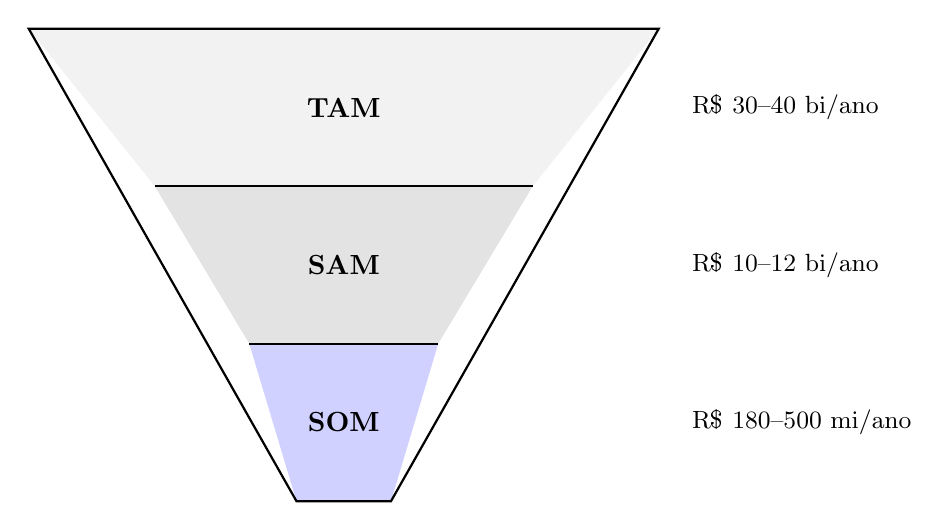
\begin{tikzpicture}[font=\small]
    \fill[gray!10]  (-4,6) -- (4,6)  -- (2.4,4) -- (-2.4,4) -- cycle;
    \fill[gray!22]  (-2.4,4) -- (2.4,4) -- (1.2,2) -- (-1.2,2) -- cycle;
    \fill[blue!18]  (-1.2,2) -- (1.2,2) -- (0.6,0) -- (-0.6,0) -- cycle;
    \draw[thick] (-4,6) -- (4,6) -- (0.6,0) -- (-0.6,0) -- cycle;
    \draw[thick] (-2.4,4) -- (2.4,4);
    \draw[thick] (-1.2,2) -- (1.2,2);
    \node[font=\bfseries] at (0,5) {TAM};
    \node[anchor=west] at (4.3,5) {R\$~30--40 bi/ano};
    \node[font=\bfseries] at (0,3) {SAM};
    \node[anchor=west] at (4.3,3) {R\$~10--12 bi/ano};
    \node[font=\bfseries] at (0,1) {SOM};
    \node[anchor=west] at (4.3,1) {R\$~180--500 mi/ano};
  \end{tikzpicture}
  \legend{Fonte: estimativas dos autores a partir de dados secundários -- a confirmar.}
\end{figure}

O TAM é o mercado odontológico privado brasileiro como um todo. O SAM considera apenas as clínicas privadas independentes com perfil de digitalização compatível com os produtos da Capim (excluindo SUS e grandes redes com sistemas próprios), partindo de um universo estimado de 80 a 100 mil clínicas ativas com ticket médio mensal entre R\$~1.500 e R\$~10.000. O SOM considera uma penetração de 3\% a 5\% dessas clínicas em cinco anos -- entre 2.500 e 5.000 clínicas ativas, ticket médio ponderado entre R\$~6.000 e R\$~10.000 mensais --, meta plausível dado o crescimento atual da base e o aumento de ticket proporcionado pelo produto POS.

A Capim opera em um setor estruturalmente atraente pelo tamanho do mercado odontológico privado, pelo momentum do ecossistema brasileiro de healthtechs e pela convergência com o mercado de fintechs. Esse posicionamento no cruzamento dos dois ecossistemas amplia o SAM endereçável em relação a concorrentes que atuam em apenas um vetor -- software, parcelamento ou maquininha isoladamente.

\section{Principais Concorrentes}

A Capim compete em três frentes simultâneas, pois seu modelo une software de gestão (SaaS), parcelamento ao paciente (BNPL) e adquirência (POS). Isso significa que a empresa não enfrenta um único concorrente direto que replique essa combinação, mas diferentes competidores em cada camada do produto.

\subsection{Concorrentes no SaaS de gestão odontológica}

O mercado brasileiro de software para clínicas odontológicas é fragmentado, com alguns players consolidados e muitos sistemas de nicho. Os dois líderes são o Simples Dental e o Clinicorp. O Simples Dental é descrito como o maior software odontológico da América Latina, com mais de 60 mil dentistas cadastrados no Brasil, diferencial de interface simples e automação de comunicação via WhatsApp, mais forte em clínicas pequenas e médias. O Clinicorp se posiciona como o sistema mais completo do mercado, com módulos de CRM, funil de vendas, gestão financeira avançada, controle multiunidade e integração com IA para análise de dados, atendendo mais de 57 mil usuários ativos, voltado a clínicas estruturadas e redes com múltiplas unidades. Outros players relevantes são o Dental Office, voltado a clínicas de médio porte com foco em controle financeiro e agendamento, e o Codental, mais direcionado a consultórios individuais.

\subsection{Concorrentes no BNPL e adquirência}

O Simples Dental oferece integração com a Parcela Mais, fintech especializada em crédito para saúde. O Clinicorp oferece funcionalidade similar por meio do Clinipay, sua solução própria de pagamentos. Outras fintechs de crédito para saúde, como KonsigaPay, EFIC e Finnsaúde, também atuam nesse espaço, mas sem integração nativa com software de gestão. Existem ainda concorrentes generalistas em BNPL, como Koin e Qista, sem produto especializado para odontologia. No produto de maquininha, a Capim compete com players generalistas de adquirência como Stone, PagSeguro e InfinitePay, que têm vantagens estruturais de escala e taxas, mas não têm especialização em odontologia nem integração com a rotina clínica.

\subsection{Síntese competitiva}

% TODO(equipe): complementar esta seção com uma análise de concorrentes nos moldes da aula 3 (material a inserir por quem participou da aula).
A Tabela~\ref{tab:concorrentes} resume o posicionamento dos principais players nas três camadas de produto.

\begin{table}[h]
  \centering
  \caption{Comparativo de concorrentes por camada de produto}
  \label{tab:concorrentes}
  \begin{tabular}{lccc}
    \toprule
    \textbf{Empresa} & \textbf{SaaS de gestão} & \textbf{BNPL nativo} & \textbf{POS integrado} \\
    \midrule
    Capim            & Sim & Sim            & Sim            \\
    Simples Dental   & Sim & Via parceiro   & Não            \\
    Clinicorp        & Sim & Via Clinipay   & Via Clinipay   \\
    Dental Office    & Sim & Não            & Não            \\
    Stone / PagSeguro& Não & Não            & Sim            \\
    \bottomrule
  \end{tabular}
  \legend{Fonte: elaborado pelos autores a partir de dados secundários (2026).}
\end{table}

Nenhum concorrente combina os três produtos com a profundidade da Capim. O Clinicorp é o player mais próximo em abrangência, mas seu produto financeiro funciona como uma camada adicional sobre o software, sem análise de crédito proprietária e sem exposição direta ao risco de inadimplência como faz a Capim.

\section{Posicionamento da Capim}

A Capim se posiciona como a única plataforma do mercado brasileiro que oferece, de forma nativa e integrada, gestão de clínica, parcelamento ao paciente e adquirência. Fundada em 2021 por Marcelo Lutz e Roberto Biselli, a empresa se define como um ERP especializado em odontologia, com camada financeira embarcada. Em fevereiro de 2025, captou uma Série A de R\$~132 milhões liderada por Valor Capital e QED Investors, com participação de ONE.VC, Canary, NXTP, Endeavor, Saison e Actyus -- este último conduzido por Sérgio Furio, CEO da Creditas. Em 2024, a receita triplicou e a base de clínicas passou a casa dos 6 mil, com o objetivo declarado de alcançar 10 mil clínicas ativas. \footnote{Dados de fundação, captação e investidores são informações institucionais/de mercado, não relatadas pelo entrevistado -- a equipe deve confirmar a exatidão e a fonte antes da entrega final.}

\subsection{Principal diferencial}

O diferencial central da Capim é assumir o risco de crédito do paciente diretamente, em vez de apenas intermediar a transação. Quando um financiamento é fechado, a clínica recebe à vista e a Capim fica responsável por toda a cobrança e pela inadimplência, sem direito de regresso contra a clínica em tratamentos já executados. Isso muda a economia da clínica, que deixa de carregar carteira de recebíveis e ganha previsibilidade de caixa, e cria para a Capim um ativo financeiro proprietário, baseado em dados próprios de comportamento de pagamento que se acumulam a cada operação.

A combinação SaaS, BNPL e POS no mesmo ambiente gera três efeitos competitivos importantes: eleva o ticket médio por clínica (mensalidade, taxa sobre TPV e spread sobre parcelamento); aumenta o custo de troca, já que sair da Capim implica trocar três fornecedores simultaneamente; e cria um ciclo de dados próprio, no qual o comportamento financeiro de pacientes e clínicas alimenta o motor de crédito e o produto de gestão -- loop que concorrentes de vetor único não conseguem replicar.

\subsection{Tecnologias e capacidades técnicas}

A plataforma é 100\% \textit{online}, acessível por celular, tablet ou computador, e segue os requisitos da LGPD. Suas principais capacidades técnicas são: um motor de análise de crédito proprietário, que consulta Serasa e Boa Vista e gera um Score Capim próprio em tempo real; um sistema de parcelamento em até 36 vezes, com juros aproximadamente 50\% menores que os praticados por bancos tradicionais para crédito ao consumidor; uma régua de cobrança automatizada via WhatsApp, e-mail e ligação telefônica; uma camada de gestão clínica completa, integrada ao motor financeiro; um terminal POS proprietário, lançado a partir de 2025 com o capital da Série A; e uma camada de inteligência artificial em desenvolvimento, voltada à automação administrativa e à geração de alertas e sugestões para o gestor da clínica.

A Capim ocupa, assim, uma posição estratégica no cruzamento entre healthtech e fintech, em um nicho historicamente subatendido por sistemas de saúde de uso geral. Os capítulos seguintes tratam dos desafios de governar a inovação dentro dessa posição.

% ==============================================================
% CAPÍTULO 5 — ANÁLISE ORGANIZACIONAL
% ==============================================================

\chapter{Análise Organizacional}
\label{cap:analise-organizacional}

Esta seção analisa a estrutura organizacional da Capim Software a partir de quatro perspectivas complementares: hierarquia interna, Estrela de Galbraith, configuração de Mintzberg e análise SWOT. As informações têm como base a entrevista com Lucas Mathias, PM de experimentos e integrante do time fundador \cite{capimentrevista2026}, e dados secundários.

\section{Hierarquia e Ritos de Coordenação}

A Capim, com cerca de 150 colaboradores em 2026, organiza-se em squads multidisciplinares por produto, com coordenação central exercida pela Diretoria de Produto. Cada squad é autônomo na operação, mas alinhado estrategicamente por meio de dois ritos formais, sintetizados na Figura~\ref{fig:organograma} e detalhados na Tabela~\ref{tab:ritos} (Capítulo~\ref{cap:processo-decisorio}).

\begin{figure}[h]
  \caption{Organograma resumido da Capim Software}
  \label{fig:organograma}
  \centering
  \resizebox{\textwidth}{!}{%
  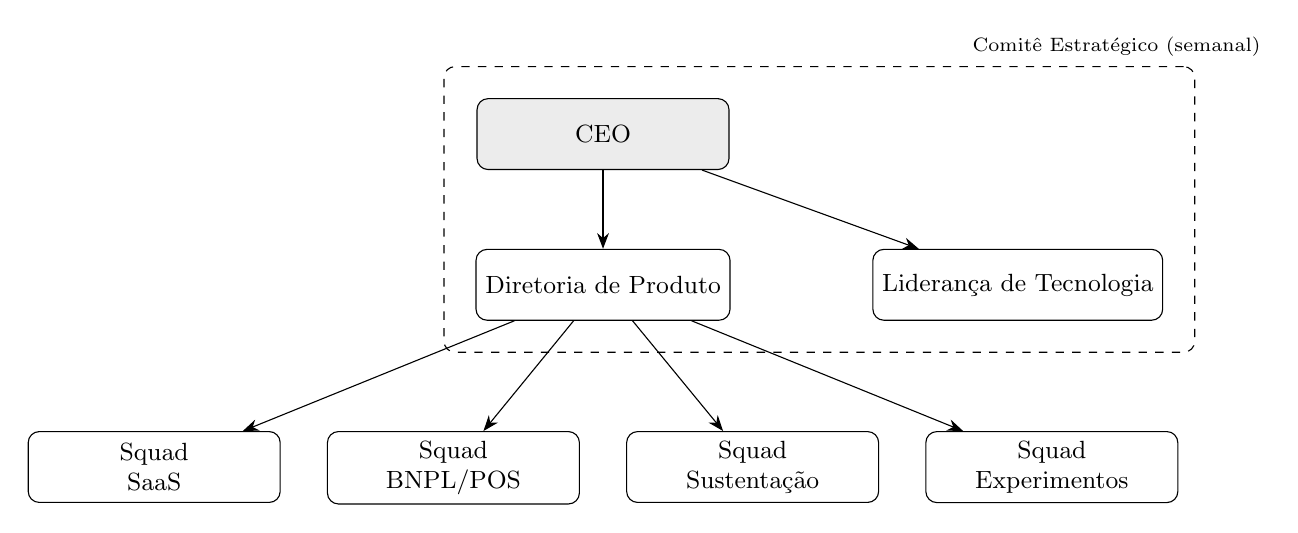
\begin{tikzpicture}[
      node distance=10mm and 6mm,
      box/.style={draw, rounded corners, align=center, minimum width=32mm, minimum height=9mm, font=\small},
      every edge/.style={draw, -{Stealth[length=2mm]}}
    ]
    \node[box, fill=gray!15] (ceo) {CEO};
    \node[box, below=of ceo] (dp) {Diretoria de Produto};
    \node[box, right=18mm of dp] (tech) {Liderança de Tecnologia};

    \node[box, below=14mm of dp, xshift=-57mm] (saas) {Squad\\SaaS};
    \node[box, below=14mm of dp, xshift=-19mm] (bnpl) {Squad\\BNPL/POS};
    \node[box, below=14mm of dp, xshift=19mm] (sust) {Squad\\Sustentação};
    \node[box, below=14mm of dp, xshift=57mm] (exp) {Squad\\Experimentos};

    \draw (ceo) edge (dp);
    \draw (ceo) edge (tech);
    \draw (dp) edge (saas);
    \draw (dp) edge (bnpl);
    \draw (dp) edge (sust);
    \draw (dp) edge (exp);

    \node[draw, dashed, rounded corners, fit=(ceo)(dp)(tech), inner sep=4mm, label={[font=\scriptsize]above right:Comitê Estratégico (semanal)}] {};
  \end{tikzpicture}}
  \legend{Fonte: elaborado pelos autores. Os squads de Sustentação e Experimentos e os ritos de coordenação são confirmados pela entrevista; a separação SaaS/BNPL-POS é uma reconstrução dos autores a partir das linhas de produto descritas, não um organograma oficial da empresa.}
\end{figure}

\section{Estrela de Galbraith}
\label{sec:galbraith}

O modelo de Galbraith avalia o alinhamento entre cinco dimensões organizacionais, classicamente representadas como uma estrela de cinco pontas (Figura~\ref{fig:galbraith-estrela}). A análise para a Capim em cada uma delas é detalhada a seguir.

\begin{figure}[h]
  \caption{As cinco dimensões da Estrela de Galbraith}
  \label{fig:galbraith-estrela}
  \centering
  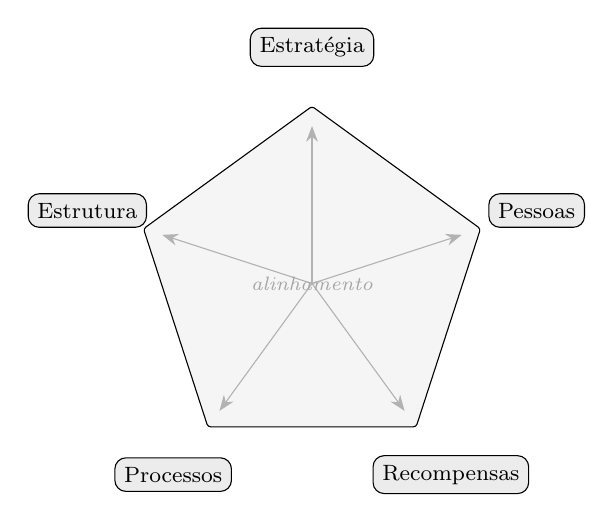
\begin{tikzpicture}[font=\small]
    \node[regular polygon, regular polygon sides=5, draw, minimum size=4.5cm,
          fill=gray!8, rounded corners=1pt] (p) {};
    \foreach \ang/\name in {90/Estratégia, 162/Estrutura, 234/Processos,
                            306/Recompensas, 18/Pessoas} {
      \node[draw, rounded corners, fill=gray!15, font=\footnotesize]
            at (\ang:3.0cm) {\name};
      \draw[-{Stealth[length=2mm]}, gray!60] (p.center) -- (\ang:2.0cm);
    }
    \node[font=\scriptsize\itshape, gray!70] at (p.center) {alinhamento};
  \end{tikzpicture}
  \legend{Fonte: elaborado pelos autores a partir do modelo de Galbraith.}
\end{figure}

\begin{description}
  \item[Estratégia] Aprofundar penetração em odontologia via ecossistema integrado (crédito + gestão + maquininha + carnê). Foco em ``agenda cheia e rentável'' para clínicas. Crescimento por dois caminhos: melhorias incrementais nos produtos existentes e \textit{home runs} experimentais (como o modelo B2C).
  \item[Estrutura] Squads autônomos por produto, com coordenação central da Diretoria de Produto. Organização enxuta (\textasciitilde150 pessoas) e horizontal nas decisões operacionais.
  \item[Processos] Combinação adaptada de Scrum (\textit{sprints}, \textit{boards}) com \textit{stage-gates} internos: Garagem~2 $\rightarrow$ Garagem~1 $\rightarrow$ Rua. Progressão controlada pelo número de clínicas expostas (5--10 $\rightarrow$ 50--100 $\rightarrow$ 500+). Métrica de sucesso por iniciativa, revisável durante o projeto.
  \item[Recompensas] Tema não aprofundado na entrevista. Indícios apontam para reconhecimento por autonomia, \textit{ownership} e exposição direta a problemas estratégicos junto ao CEO.
  \item[Pessoas] Entrevistado e fundadores com passagem por MBA fora do Brasil, segundo relato. Cultura de iteração rápida, uso intensivo de IA (Claude, Cursor) e proximidade com o usuário final.
\end{description}

As cinco dimensões mostram-se majoritariamente alinhadas: estratégia experimental sustentada por estrutura enxuta, processos adaptáveis e pessoas culturalmente engajadas. A dimensão de processos, contudo, é examinada com maior profundidade no Capítulo~\ref{cap:processo-decisorio}, onde se mostra que o mesmo arranjo de \textit{stage-gates} adaptado é aplicado de forma relativamente uniforme a projetos de incerteza muito distinta.

\section{Configuração de Mintzberg}
\label{sec:mintzberg}

A análise indica que a Capim se enquadra majoritariamente como adhocracia operacional, configuração típica de organizações cuja atividade central é a inovação. O mecanismo de coordenação predominante é o ajuste mútuo, exercido por meio das reuniões quinzenais e semanais já descritas, em detrimento da padronização rígida de processos. A parte-chave da organização é o núcleo operacional -- os times de produto --, com forte assessoria de apoio em design, engenharia e funções de suporte. Em termos de parâmetros de design, a empresa apresenta estrutura orgânica, especialização horizontal, dispositivos de ligação entre squads e descentralização seletiva das decisões. Os fatores contextuais reforçam esse enquadramento: ambiente dinâmico, tecnologia sofisticada (software e IA) e uma organização ainda jovem, de porte médio.

Há uma exceção: o squad de sustentação apresenta traços mais burocráticos, com fluxos de trabalho mais previsíveis. Ainda assim, mesmo essa equipe se engaja em inovações incrementais, como a migração automática de sistemas legados, o que mantém a adhocracia como configuração dominante na empresa como um todo.

\section{Análise SWOT}
\label{sec:swot}

A Figura~\ref{fig:swot-quadrante} sintetiza os pontos centrais da análise no formato clássico de quadrante; a Tabela~\ref{tab:swot} detalha a lista completa.

\begin{figure}[h]
  \caption{Síntese da análise SWOT da Capim}
  \label{fig:swot-quadrante}
  \centering
  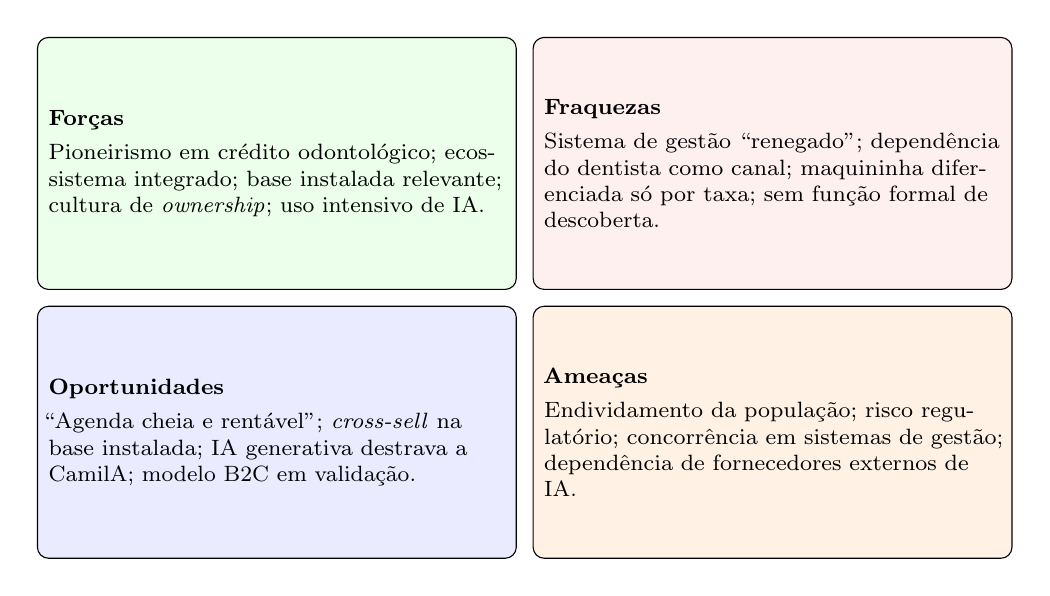
\begin{tikzpicture}[font=\footnotesize,
      cell/.style={draw, rounded corners, text width=58mm, align=left,
                   inner sep=4pt, minimum height=32mm}]
    \matrix[row sep=2mm, column sep=2mm] {
      \node[cell, fill=green!8] {\textbf{Forças}\par\smallskip
        Pioneirismo em crédito odontológico; ecossistema integrado; base instalada relevante; cultura de \textit{ownership}; uso intensivo de IA.}; &
      \node[cell, fill=red!6] {\textbf{Fraquezas}\par\smallskip
        Sistema de gestão ``renegado''; dependência do dentista como canal; maquininha diferenciada só por taxa; sem função formal de descoberta.}; \\
      \node[cell, fill=blue!8] {\textbf{Oportunidades}\par\smallskip
        ``Agenda cheia e rentável''; \textit{cross-sell} na base instalada; IA generativa destrava a CamilA; modelo B2C em validação.}; &
      \node[cell, fill=orange!10] {\textbf{Ameaças}\par\smallskip
        Endividamento da população; risco regulatório; concorrência em sistemas de gestão; dependência de fornecedores externos de IA.}; \\
    };
  \end{tikzpicture}
  \legend{Fonte: elaborado pelos autores a partir da entrevista com Lucas Mathias (2026). Versão completa na Tabela~\ref{tab:swot}.}
\end{figure}

\begin{table}[h]
  \centering
  \caption{Análise SWOT da Capim -- detalhamento}
  \label{tab:swot}
  \begin{tabularx}{\textwidth}{XX}
    \toprule
    \textbf{Forças} & \textbf{Fraquezas} \\
    \midrule
    Pioneirismo em crédito odontológico no ponto de venda &
    Sistema de gestão tratado internamente como produto ``renegado'' \\
    Ecossistema integrado (crédito, gestão, maquininha, carnê) &
    Dependência do dentista como canal de venda do crédito \\
    Base instalada: 6.000+ clínicas, R\$~450M+ em crédito originado, 70 mil+ pacientes &
    Maquininha diferenciada principalmente por taxa \\
    Cultura de \textit{ownership} e capacidade de iteração rápida &
    Portfólio concentrado em uma única vertical (odontologia) \\
    Uso intensivo de IA no produto e na operação interna &
    Iniciativas congeladas aguardando maturação tecnológica (caso CamilA) \\
    Time fundador qualificado e ainda atuante na empresa &
    Ausência de função formal de descoberta/geração de ideias (ver Capítulo~\ref{cap:processo-decisorio}) \\
    \bottomrule
  \end{tabularx}

  \vspace{2mm}
  \begin{tabularx}{\textwidth}{XX}
    \toprule
    \textbf{Oportunidades} & \textbf{Ameaças} \\
    \midrule
    Aumentar receita das clínicas via aquisição de pacientes (``agenda cheia e rentável'') &
    Endividamento da população limita a base elegível ao crédito \\
    \textit{Cross-sell} na base instalada de 6.000+ clínicas &
    Risco regulatório em crédito e meios de pagamento \\
    Avanços em IA generativa destravam iniciativas como a CamilA &
    Concorrência intensa em sistemas de gestão odontológica \\
    Expansão para verticais adjacentes (ótica, medicina geral, cirurgias eletivas) &
    Pressão sobre margens da maquininha \\
    Modelo B2C (``Uber dos dentistas'') em validação &
    Dependência de fornecedores externos de IA (Anthropic, OpenAI) \\
    Aprimoramento de modelos de risco para ampliar a aprovação responsável &
    Exposição ao macroambiente (``metáfora do elefante'' relatada pelo entrevistado) \\
    \bottomrule
  \end{tabularx}
  \legend{Fonte: elaborado pelos autores a partir da entrevista com Lucas Mathias (2026).}
\end{table}

A Capim conjuga liderança consolidada em sua categoria pioneira (crédito odontológico) com a necessidade de diversificar canais e produtos para mitigar a dependência do dentista como intermediário e a exposição ao cenário macroeconômico. Os capítulos seguintes mostram que parte dessas fraquezas e ameaças, em particular a ausência de uma função formal de descoberta de oportunidades, está diretamente relacionada a lacunas no próprio sistema de gestão da inovação da empresa.

% ==============================================================
% CAPÍTULO 6 — ANÁLISE DO PROCESSO DECISÓRIO DE INOVAÇÃO
% ==============================================================

\chapter{Análise do Processo Decisório de Inovação}
\label{cap:processo-decisorio}

Este é o capítulo central do relatório. Diferentemente da versão anterior do trabalho -- em que o processo decisório foi descrito de forma majoritariamente narrativa --, esta versão aplica diretamente ao caso da Capim os quatro frameworks de gestão da inovação apresentados na Seção~\ref{cap:metodologia}: a tipologia contingencial de processos de inovação, a cadeia de valor da inovação, a gestão de portfólio por risco e retorno, e o modelo de ambidestria Descoberta--Incubação--Aceleração.

\section{Visão Geral do Processo Decisório Atual}

A Capim não utiliza nenhum sistema formal e documentado de gestão da inovação, do tipo manual de processos ou metodologia com nome próprio. Sua governança da inovação combina, de forma pragmática, princípios ágeis de desenvolvimento de software com uma lógica própria de estágios sucessivos, inspirada em -- mas não idêntica a -- modelos clássicos de \textit{stage-gates} \cite{cooper1990}.

\subsection{Participantes e comitês}

A governança da inovação na Capim é desenhada para dar autonomia aos times, mantendo o alinhamento estratégico da liderança, por meio de quatro grupos de responsabilidade:

\begin{description}
  \item[Times de produto autônomos] cada squad foca em iterar e construir funcionalidades de forma ágil para seu produto.
  \item[Diretoria de Produto] coordenação centralizada cujo papel principal é evitar interferências e sobreposições de trabalho entre squads.
  \item[Comitê tático] reuniões quinzenais com todos os PMs e o time de design, para sincronização do desenvolvimento.
  \item[Comitê estratégico] reunião semanal entre CEO, Diretoria de Produto, liderança de tecnologia e o PM de experimentos, na qual se definem rumos e se tratam problemas críticos.
\end{description}

\subsection{Pontos de decisão e gates}

O ciclo de vida dos projetos experimentais segue uma adaptação própria de \textit{stage-gates}, em que o avanço de um projeto desencadeia o envolvimento progressivo do restante da organização (Tabela~\ref{tab:gates}). A progressão entre estágios é controlada pelo número de clínicas parceiras expostas ao experimento -- de 5--10, para 50--100, até cerca de 500 --, e não por um calendário fixo.

\begin{table}[H]
  \centering
  \caption{Estágios do processo decisório da Capim}
  \label{tab:gates}
  \begin{tabularx}{\textwidth}{lXX}
    \toprule
    \textbf{Estágio} & \textbf{Características} & \textbf{Times envolvidos} \\
    \midrule
    Garagem 2 & Maior incerteza. Time isolado testa hipóteses sem impactar a operação geral. 5--10 clínicas parceiras. & Produto (isolado) \\
    Garagem 1 & Estágio intermediário de transição e evolução do experimento. 50--100 clínicas expostas. & Produto + marketing + engenharia \\
    Rua & Produto maduro, lançado e tratado como item de prateleira. 500+ clínicas. & + onboarding, suporte e comercial \\
    \bottomrule
  \end{tabularx}
  \legend{Fonte: elaborado pelos autores a partir da entrevista com Lucas Mathias (2026).}
\end{table}

\subsection{Critérios de decisão e gestão da incerteza}

Os critérios de \textit{go/no-go} para manter, cancelar ou pausar um projeto não dependem de um ciclo de vida estável -- a Capim não trata nenhum produto como estando em ``mera manutenção''. Em vez disso, adota três mecanismos:

\begin{enumerate}
  \item \textbf{Métrica de sucesso específica por iniciativa}, definida no início de cada projeto e revisável ao longo da execução -- por exemplo, o projeto de aquisição B2C de pacientes mudou sua métrica-alvo de ``contratos de crédito assinados'' para ``tratamentos fechados pelas clínicas parceiras'' após aprendizado empírico sobre o que de fato gerava valor.
  \item \textbf{Ciclos trimestrais de avaliação}, com disciplina organizacional de não desistir prematuramente -- a equipe ``luta pelo projeto até o fim do trimestre''.
  \item \textbf{Congelamento \textit{versus} descontinuação}: se o projeto falha no trimestre, pode ser desligado e documentado, ou ``congelado'' aguardando maturação tecnológica -- como ocorreu com a CamilA, assistente de IA que continua ativa para as clínicas que já a utilizam, mas sem novos investimentos de desenvolvimento.
\end{enumerate}

Essa descrição, por si só, já indica uma governança mais sofisticada do que a simples ausência de processo. As seções a seguir avaliam essa governança à luz dos frameworks da disciplina.

\section{Classificação pela Tipologia de Processos de Inovação}
\label{sec:tipologia}

\textcite{salerno2015} argumentam, a partir de teoria contingencial, que não existe um único processo ``correto'' de inovação aplicável a qualquer projeto: o processo adequado depende do grau de incerteza de mercado e de tecnologia e do papel do cliente na especificação da solução. Os autores propõem uma tipologia de oito processos, dos quais quatro são particularmente relevantes para a Capim: o processo \textit{tradicional} (da ideia ao lançamento, adequado a inovações incrementais em mercado e tecnologia maduros); o processo de \textit{atividades paralelas} (em que a comercialização começa antes de o desenvolvimento estar concluído, típico de software); e os processos de \textit{pausa} -- esperando o mercado, esperando a tecnologia, ou ambos -- em que o projeto é deliberadamente suspenso até que uma condição externa se resolva.

Ao classificar as linhas de produto da Capim segundo essa tipologia (Tabela~\ref{tab:tipologia}), observa-se que a empresa, na prática, já opera mais de um tipo de processo simultaneamente -- mas sem reconhecer essa diferença formalmente na governança.

\begin{table}[H]
  \centering
  \caption{Classificação das iniciativas da Capim segundo a tipologia de \textcite{salerno2015}}
  \label{tab:tipologia}
  \begin{tabularx}{\textwidth}{lXX}
    \toprule
    \textbf{Iniciativa} & \textbf{Tipo de processo predominante} & \textbf{Implicação} \\
    \midrule
    Sistema de gestão (lembretes, melhorias incrementais) & Tradicional (idea-to-launch) & Mercado e tecnologia maduros; \textit{stage-gates} trimestrais são adequados. \\
    Capix (crédito via Pix) & Tradicional, com elementos de atividades paralelas & Incerteza baixa; lançamento incremental sobre fluxo já existente (WhatsApp $\rightarrow$ interface dedicada). \\
    CamilA (IA conversacional de vendas) & Pausa esperando avanço tecnológico + atividades paralelas & Tratada na prática como projeto tradicional com métrica trimestral fixa; a tipologia indica que deveria ser formalmente reconhecida como \textit{pausa ativa}, não como falha do processo tradicional. \\
    Modelo B2C (``Uber dos dentistas'') & Pausa esperando o mercado / atividades paralelas & Alta incerteza de mercado (resposta de clínicas e pacientes a um modelo de relação inédito); aplicar o mesmo ciclo trimestral rígido do processo tradicional tende a subestimar o tempo de aprendizado necessário. \\
    \bottomrule
  \end{tabularx}
  \legend{Fonte: elaborado pelos autores.}
\end{table}

O ponto central deste diagnóstico é que a Capim aplica essencialmente \textbf{um único regime de governança} -- métrica por iniciativa mais ciclo trimestral de \textit{go/no-go} -- a projetos que, pela tipologia de \textcite{salerno2015}, pertencem a categorias de processo distintas. Isso é particularmente visível no caso da CamilA: o relato da entrevista descreve o desfecho do projeto como um ``congelamento'' decidido ao fim do ciclo trimestral por não atingimento da métrica -- mas a causa-raiz apontada pelo próprio entrevistado é a imaturidade da tecnologia de IA generativa disponível no período, ou seja, exatamente a condição que define um processo de \textit{pausa esperando avanço tecnológico}. Sem o reconhecimento formal desse tipo de processo, a empresa corre o risco de reavaliar a CamilA nos próximos ciclos com o mesmo critério financeiro/de adoção que usaria para um produto maduro, em vez de um critério de prontidão tecnológica.

\section{Diagnóstico pela Cadeia de Valor da Inovação}
\label{sec:cadeia-valor}

\textcite{hansenbirkinshaw2007} propõem enxergar a inovação como uma cadeia de valor de três elos -- \textit{geração de ideias} (interna, entre unidades e externa), \textit{conversão} (seleção, financiamento e desenvolvimento) e \textit{difusão} (disseminação pela organização) -- e argumentam que a capacidade de inovação de uma empresa é limitada pelo elo mais fraco da cadeia, não pela média dos três.

Aplicando esse diagnóstico à Capim:

\begin{description}
  \item[Conversão -- elo forte.] A empresa possui um mecanismo claro de seleção e financiamento: métricas de sucesso por iniciativa, ciclos trimestrais de avaliação e critérios diferenciados para congelamento \textit{versus} descontinuação. Squads autônomos com orçamento e mandato próprio desenvolvem as iniciativas selecionadas.
  \item[Difusão -- elo forte.] A progressão controlada por número de clínicas expostas (5--10 $\rightarrow$ 50--100 $\rightarrow$ 500+) é, em essência, um mecanismo de difusão gradual e deliberado, que aciona times de suporte, onboarding e comercial apenas quando o produto está maduro para tanto -- evitando o despreparo organizacional.
  \item[Geração de ideias -- elo não evidenciado.] Em nenhum momento da entrevista foi descrito um mecanismo formal de captação ou geração de ideias -- nem interno (mecanismos de polinização cruzada entre squads), nem externo (escuta estruturada de clínicas, dentistas ou parceiros de tecnologia). As iniciativas mencionadas (Capix, CamilA, modelo B2C) parecem emergir de decisões da liderança ou de oportunidades identificadas de forma ad hoc pelo PM de experimentos, e não de um processo sistemático de descoberta.
\end{description}

Esse diagnóstico responde diretamente à pergunta levantada na devolutiva do professor sobre se a empresa tem um problema de geração de ideias: \textbf{sim, há indícios de que esse é o elo mais fraco da cadeia de valor da inovação da Capim}. A empresa investiu em mecanismos sofisticados de conversão e difusão, mas não em um mecanismo equivalente de geração e descoberta de oportunidades -- o que é desenvolvido com mais detalhe no Capítulo~\ref{cap:diagnostico-proposta}.

\section{Portfólio de Inovação: Risco e Retorno}
\label{sec:portfolio}

\textcite{goffinmitchell2010} propõem avaliar o portfólio de projetos de inovação por meio de uma matriz de risco e retorno, classificando iniciativas em quatro quadrantes: \textit{Pearls} (alto retorno, baixa incerteza), \textit{Oysters} (alto retorno, alta incerteza), \textit{White Elephants} (baixo retorno, alta incerteza) e \textit{Bread and Butter} (baixo retorno, baixa incerteza -- tipicamente projetos incrementais).

\begin{table}[H]
  \centering
  \caption{Carteira de iniciativas da Capim na matriz risco-retorno}
  \label{tab:portfolio}
  \begin{tabularx}{\textwidth}{lXX}
    \toprule
    \textbf{Quadrante} & \textbf{Iniciativas da Capim} & \textbf{Leitura} \\
    \midrule
    Bread and Butter (baixo risco, retorno previsível) & Sistema de gestão (melhorias incrementais), Capix & Núcleo de manutenção e melhoria contínua da base instalada; bem servido pelo processo tradicional de \textit{stage-gates}. \\
    Oysters (alto risco, alto retorno potencial) & CamilA, modelo B2C (``Uber dos dentistas'') & \textit{Home runs} aguardando validação; exigem tolerância a incerteza prolongada e critérios de avaliação não puramente financeiros. \\
    White Elephants (alto risco, retorno incerto) & Iniciativas descontinuadas sem registro sistemático (mencionadas apenas informalmente como ``deu errado'') & Risco de a empresa não capturar aprendizado de projetos encerrados, por falta de documentação estruturada. \\
    Pearls (baixo risco, alto retorno) & Não identificado claramente no relato & Possível sinal de que o portfólio carece de iniciativas já validadas tecnicamente, mas ainda não escaladas -- typically alimentadas por um funil de descoberta robusto. \\
    \bottomrule
  \end{tabularx}
  \legend{Fonte: elaborado pelos autores a partir da entrevista com Lucas Mathias (2026).}
\end{table}

A ausência de iniciativas claramente classificáveis como \textit{Pearls} reforça o diagnóstico da Seção~\ref{sec:cadeia-valor}: sem um funil de descoberta que amadureça oportunidades de baixo risco e alto retorno antes de irem a mercado, o portfólio da Capim tende a se polarizar entre projetos incrementais de baixo risco (\textit{Bread and Butter}) e apostas radicais de alto risco (\textit{Oysters}), sem o estágio intermediário que tipicamente preencheria o quadrante de \textit{Pearls}.

\section{Ambidestria: Descoberta, Incubação e Aceleração}
\label{sec:ambidestria}

\textcite{salernogomes2018} descrevem o modelo de três macroatividades -- Descoberta, Incubação e Aceleração (DNA) -- segundo o qual sistemas de gestão da inovação mais radical precisam diferenciar explicitamente a governança de cada fase, em vez de tratar toda inovação com o mesmo processo. Mapeando os estágios da Capim a esse modelo (Tabela~\ref{tab:dna}):

\begin{table}[H]
  \centering
  \caption{Estágios da Capim mapeados ao modelo Descoberta-Incubação-Aceleração}
  \label{tab:dna}
  \begin{tabularx}{\textwidth}{lXX}
    \toprule
    \textbf{Macroatividade} & \textbf{Equivalente na Capim} & \textbf{Observação} \\
    \midrule
    Descoberta & \textbf{Não formalizada} & Não há hub, função ou rito dedicado à busca ativa de oportunidades antes da Garagem~2; o projeto já ``nasce'' como hipótese a testar. \\
    Incubação & Garagem 2 & Time isolado testa hipóteses com 5--10 clínicas parceiras, protegido da operação corrente. \\
    Aceleração & Garagem 1 $\rightarrow$ Rua & Envolvimento progressivo de marketing, engenharia, suporte e comercial conforme a base de clínicas expostas cresce. \\
    \bottomrule
  \end{tabularx}
  \legend{Fonte: elaborado pelos autores a partir de \textcite{salernogomes2018} e da entrevista com Lucas Mathias (2026).}
\end{table}

A Capim, portanto, já pratica uma forma de ambidestria estrutural ao isolar a Garagem~2 do restante da operação -- mecanismo equivalente ao que \textcite{hansenbirkinshaw2007} chamam de ``\textit{safe haven}'' para a fase de conversão. O que está ausente é a etapa de \textbf{Descoberta} propriamente dita: segundo \textcite{salernogomes2018}, geração de ideias tradicional (sugestão avaliada em um comitê) não equivale a Descoberta, que envolve visão simultânea de oportunidade de mercado e plataforma tecnológica, tipicamente sustentada por uma função ou ``hub'' de inovação dedicado. \textcite{oconnormeyer2026} chegam à mesma conclusão a partir de pesquisa mais recente: tratar a inovação estratégica como função permanente -- com Descoberta como competência organizacional dedicada, e não apenas como etapa implícita antes da incubação.

Adicionalmente, tanto \textcite{salernogomes2018} quanto \textcite{oconnormeyer2026} enfatizam que projetos incrementais e radicais devem ser geridos por sistemas de decisão \textbf{diferentes} -- não apenas por equipes diferentes. Na Capim, a separação de equipes (squads \textit{versus} Garagem~2) já existe, mas os \textbf{critérios de decisão} permanecem os mesmos para ambos os tipos de projeto: uma métrica quantitativa fixada no início e avaliada ao fim do trimestre. \textcite{salernogomes2018} mostram, a partir de casos reais, que aplicar critérios financeiros ou de adoção típicos do processo tradicional a projetos de alta incerteza tende a gerar decisões equivocadas de descontinuação precoce -- risco que se materializa no caso da CamilA, analisado na Seção~\ref{sec:tipologia}. Essa constatação fundamenta diretamente a proposta de adoção de um \textit{learning plan} formal, desenvolvida no Capítulo~\ref{cap:diagnostico-proposta}.

% ==============================================================
% CAPÍTULO 7 — DIAGNÓSTICO E PROPOSTA DE MELHORIA
% ==============================================================

\chapter{Diagnóstico e Proposta de Melhoria}
\label{cap:diagnostico-proposta}

\section{Pontos Negativos do Processo Atual}
\label{sec:pontos-negativos}

A aplicação dos frameworks do Capítulo~\ref{cap:processo-decisorio} ao processo decisório da Capim permite consolidar cinco pontos negativos. Os três primeiros têm maior aderência direta ao relato da entrevista; os dois últimos são inferidos a partir da ausência de menção a determinados mecanismos em uma única entrevista, e devem ser tratados como hipóteses a confirmar, não como diagnósticos fechados.

\begin{enumerate}
  \item \textbf{Ausência de uma função formal de Descoberta.} Como mostrado na Seção~\ref{sec:ambidestria}, não há, no relato, evidência de hub, rito ou responsável dedicado à busca ativa de oportunidades. Os projetos mencionados (Capix, CamilA, modelo B2C) são descritos como emergindo de percepções da liderança, não de um processo sistemático de geração e captação de ideias. Pela leitura da cadeia de valor da inovação (Seção~\ref{sec:cadeia-valor}), este é o elo mais fraco do sistema.
  \item \textbf{Estrutura de avaliação igual para projetos de incerteza distinta.} O \textit{formato} do critério -- uma métrica fixada no início e formalmente revisada ao fim do trimestre -- é aplicado da mesma forma a um produto incremental maduro (sistema de gestão) e a uma aposta radical em incubação (CamilA), ainda que o \textit{valor} da métrica varie por projeto. O acompanhamento informal do andamento de cada iniciativa também ocorre na Reunião Estratégica semanal (Tabela~\ref{tab:ritos}), mas a decisão estrutural de manter, pausar ou descontinuar um projeto permanece atrelada ao ciclo trimestral, independentemente do tipo de incerteza envolvida. A tipologia de \textcite{salerno2015} sugere que projetos de categorias de processo distintas deveriam ser avaliados com estruturas de critério também distintas, não apenas com metas diferentes dentro da mesma estrutura.
  % TODO(equipe): confirmar com o Axel se a leitura de informalidade no resourcing abaixo procede.
  \item \textbf{Possível dependência de pessoas-chave e informalidade no \textit{resourcing}.} A entrevista não relata dificuldades de orçamento ou recursos para inovação, mas também não descreve mecanismos formais e documentados de alocação de tempo, orçamento ou carreira para quem lidera iniciativas radicais -- a coordenação parece concentrada na disponibilidade do PM de experimentos e da Diretoria de Produto. \textcite{salerno2025} discutem por que mecanismos formais (e não apenas informais) tendem a ser necessários para sustentar o \textit{newstream} a partir do \textit{mainstream} de forma previsível; resta confirmar com a empresa se essa informalidade é, de fato, percebida internamente como um problema.
  % TODO(equipe): Axel lembra do entrevistado mencionar uma gestão do conhecimento mais estruturada -- confirmar na transcrição/com a empresa antes de manter esta leitura.
  \item \textbf{Registro de aprendizado pouco integrado à geração de novas ideias.} A entrevista indica que projetos descontinuados são documentados (``deixa documentado lá e pronto''), o que contradiz uma leitura de ausência total de registro. O ponto mais defensável é outro: não há evidência, no relato, de que esse registro alimente de volta um funil estruturado de novas ideias -- ele parece arquivado, não reaproveitado.
  \item \textbf{Portfólio sem visão consolidada de risco e retorno.} As decisões de continuidade são tomadas projeto a projeto, sem uma visão de carteira que avalie explicitamente o balanceamento entre iniciativas de baixo e alto risco (Seção~\ref{sec:portfolio}). Na prática, isso significa que a Reunião Estratégica semanal decide sobre cada iniciativa isoladamente -- manter, pausar ou descontinuar --, sem uma pauta periódica que examine a carteira como um todo e pergunte, por exemplo, se a empresa está excessivamente concentrada em apostas de alto risco (\textit{Oysters}) e melhorias incrementais (\textit{Bread and Butter}), sem cultivar deliberadamente oportunidades de baixo risco e alto retorno (\textit{Pearls}). Esse ponto é particularmente relevante porque uma visão de portfólio explícita tende a preceder -- e a justificar -- a própria função de Descoberta proposta na Seção~\ref{sec:sistema-proposto}: sem uma leitura periódica de onde a carteira está desbalanceada, é difícil priorizar em que tipo de oportunidade essa função deveria investir esforço de busca. A ausência de iniciativas no quadrante de \textit{Pearls} é consistente com essa lacuna, mas a amostra de apenas quatro iniciativas conhecidas limita a força dessa conclusão.
\end{enumerate}

\section{Sistema Proposto}
\label{sec:sistema-proposto}

A proposta de aprimoramento preserva os elementos do processo atual que se mostraram coerentes com a literatura -- a separação física e organizacional da Garagem~2, a progressão controlada por exposição a clínicas, e a disciplina de métricas por iniciativa -- e introduz quatro mecanismos adicionais, voltados a corrigir os pontos negativos identificados.

\subsection{Função de Descoberta de Oportunidades}

Recomenda-se a criação de uma função de Descoberta, antecedendo formalmente a Garagem~2, nos termos discutidos por \textcite{salernogomes2018} e \textcite{oconnormeyer2026}. Cabe uma ressalva de proporcionalidade antes de detalhar a proposta: para uma organização de \textasciitilde150 pessoas como a Capim, criar de imediato um ``hub'' -- uma estrutura dedicada, com equipe e orçamento próprios -- pode ser desproporcional ao estágio da empresa e correr o risco de burocratizar exatamente o processo que hoje é ágil por ser informal. A alternativa mais conservadora, adotada aqui, é começar pela atribuição de um \textbf{papel} de Descoberta a uma pessoa já existente na Diretoria de Produto (não uma nova área), com escopo e tempo protegido explícitos, evoluindo para uma estrutura mais formal apenas se o volume de oportunidades identificadas justificar a dedicação de mais recursos. Concretamente, isso significa:

\begin{itemize}
  \item Designar, dentro da Diretoria de Produto, um papel explícito de ``caçador de oportunidades'' -- não necessariamente uma nova contratação ou área --, com tempo protegido para escuta ativa de clínicas, dentistas e parceiros de tecnologia (IA, fintechs, distribuidores de equipamentos odontológicos), em vez de depender apenas de percepções emergentes do PM de experimentos.
  \item Instituir um rito leve e periódico (por exemplo, mensal) de polinização cruzada entre squads, no qual cada equipe apresenta sinais de oportunidade observados em sua frente -- mecanismo direto de geração de ideias internas, na acepção de \textcite{hansenbirkinshaw2007}.
  \item Tratar cada oportunidade identificada como um item de um portfólio de descoberta, e não como uma proposta isolada a ser aprovada ou rejeitada em uma única reunião -- alinhado à recomendação de \textcite{oconnormeyer2026} de tratar domínios de inovação estratégica como portfólios de experimentos, e não como pipeline de \textit{go/kill}.
\end{itemize}

\subsection{Learning Plan para Iniciativas em Incubação}

Para projetos que ingressam na Garagem~2 com alta incerteza de mercado e/ou tecnologia -- como foi o caso da CamilA --, recomenda-se a adoção de um \textit{learning plan} formal antes da entrada nos ciclos trimestrais de avaliação tradicionais, conforme proposto por \textcite{riceoconnorpierantozzi2008} e detalhado, com casos aplicados, por \textcite{salernogomes2018}.

O \textit{learning plan} consiste em um ciclo iterativo que parte da identificação explícita do que é conhecido e do que é desconhecido em quatro categorias de incerteza -- técnica, mercadológica, organizacional e de recursos --, avalia a criticidade relativa de cada incerteza, formula hipóteses testáveis de menor custo possível e realimenta o ciclo com o aprendizado obtido, antes de qualquer compromisso financeiro maior. Esse mecanismo ocupa, no espectro de abordagens de gestão de incerteza, uma posição mais adequada a incertezas elevadas do que os \textit{stage-gates} tradicionais ou os \textit{milestones} simples -- e é particularmente recomendável nos casos em que, como na CamilA, a causa do não atingimento da métrica trimestral é a imaturidade tecnológica, e não a falta de mérito da ideia.

Na prática, recomenda-se que a transição da Garagem~2 para a Garagem~1 deixe de ser condicionada apenas ao atingimento de uma métrica de adoção fixa e passe a exigir, adicionalmente, a conclusão satisfatória de um ciclo de \textit{learning plan} -- reduzindo o risco de descontinuar prematuramente iniciativas tecnologicamente promissoras, mas ainda imaturas.

\subsection{Diferenciação Formal de Processos por Tipo de Incerteza}

Recomenda-se que a Diretoria de Produto classifique explicitamente cada iniciativa, no momento de sua entrada na Garagem~2, segundo a tipologia de \textcite{salerno2015} (Tabela~\ref{tab:tipologia}), e associe a cada tipo um critério de avaliação coerente:

\begin{itemize}
  \item Iniciativas do tipo \textit{tradicional} (mercado e tecnologia maduros, como melhorias do sistema de gestão e do Capix) continuam no regime atual de métrica trimestral e \textit{stage-gates}.
  \item Iniciativas classificadas como \textit{pausa esperando tecnologia} ou \textit{pausa esperando mercado} (como a CamilA e o modelo B2C, respectivamente) passam a ter ciclos de avaliação vinculados a marcos de maturidade tecnológica ou de validação de mercado, e não apenas ao calendário trimestral -- evitando que o relógio do trimestre force decisões binárias sobre fenômenos que evoluem em ritmo diferente.
\end{itemize}

\subsection{Mecanismos Formais de \textit{Resourcing}}

% TODO(equipe): confirmar com o Axel se mecanismos formais desse tipo fazem sentido para uma empresa do porte da Capim (~150 pessoas), ou se uma versão mais leve é mais adequada.
Inspirando-se no caso de ambidestria estrutural documentado por \textcite{salerno2025}, recomenda-se formalizar os mecanismos pelos quais squads autônomos (\textit{mainstream}) cedem tempo, orçamento e pessoas para iniciativas em incubação (\textit{newstream}): acordos explícitos de alocação de horas de engenharia por trimestre, um orçamento anual dedicado a experimentos da Garagem~2 independente do orçamento operacional dos squads, e critérios de carreira e reconhecimento específicos para quem lidera iniciativas de alta incerteza -- de modo que o sucesso nessas funções não seja avaliado pelas mesmas métricas de entrega usadas para produtos maduros. Dado o porte ainda enxuto da empresa (\textasciitilde150 colaboradores), esses acordos podem começar de forma simples -- por exemplo, um percentual fixo e pequeno da capacidade de engenharia reservado por trimestre --, evoluindo em formalidade apenas na medida em que o número de iniciativas em incubação crescer.

\subsection{Portfólio de Inovação com Revisão Periódica}

Por fim, recomenda-se que a Reunião Estratégica semanal passe a revisar, periodicamente (por exemplo, a cada trimestre), uma visão consolidada da carteira de iniciativas na matriz de risco e retorno de \textcite{goffinmitchell2010} (Tabela~\ref{tab:portfolio}), de modo a tornar explícito o balanceamento entre projetos \textit{Bread and Butter} e \textit{Oysters}, e a identificar deliberadamente a necessidade de desenvolver iniciativas no quadrante de \textit{Pearls} -- oportunidades de baixo risco e alto retorno, tipicamente amadurecidas pela própria função de Descoberta proposta na Seção anterior.

\section{Síntese da Proposta}

A Figura~\ref{fig:antes-depois} e a Tabela~\ref{tab:sintese-proposta} resumem a transição proposta do sistema atual para o sistema aprimorado.

\begin{figure}[h]
  \caption{Transição proposta: sistema atual \textit{versus} sistema aprimorado}
  \label{fig:antes-depois}
  \centering
  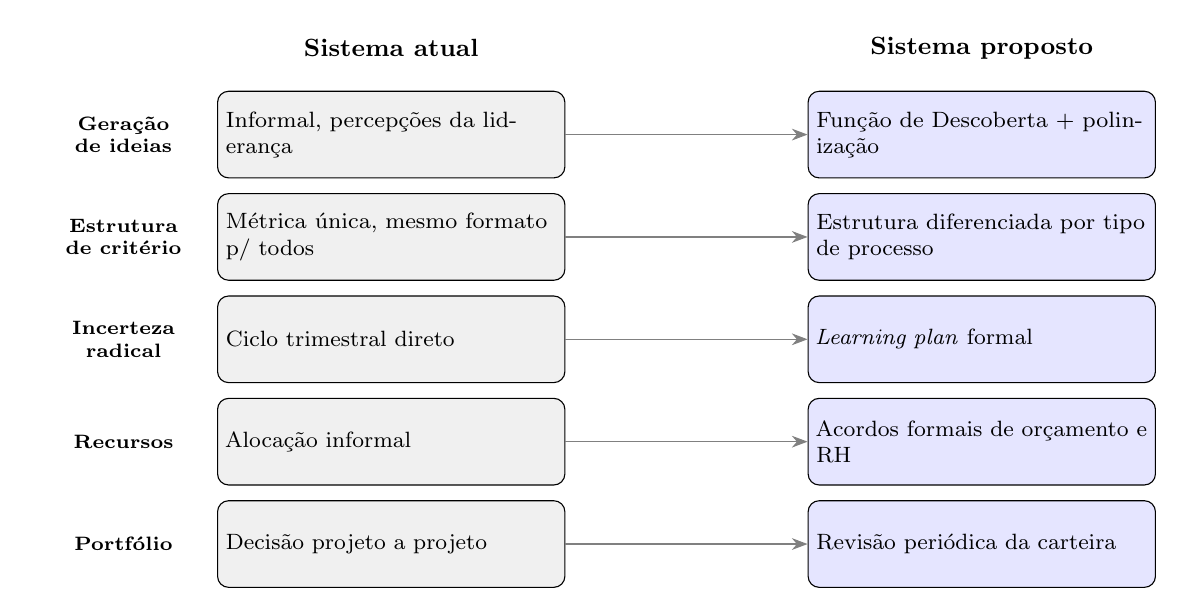
\begin{tikzpicture}[
      font=\footnotesize, node distance=2mm,
      now/.style={draw, fill=gray!12, rounded corners, text width=42mm, align=left, inner sep=3pt, minimum height=11mm},
      new/.style={draw, fill=blue!10, rounded corners, text width=42mm, align=left, inner sep=3pt, minimum height=11mm},
      dim/.style={font=\scriptsize\bfseries, align=center, text width=22mm}
    ]
    \node[font=\small\bfseries] (h1) at (0,1.1) {Sistema atual};
    \node[font=\small\bfseries] (h2) at (7.5,1.1) {Sistema proposto};
    \foreach \i/\d/\a/\b in {
      0/Geração de ideias/{Informal, percepções da liderança}/{Função de Descoberta + polinização},
      1/Estrutura de critério/{Métrica única, mesmo formato p/ todos}/{Estrutura diferenciada por tipo de processo},
      2/Incerteza radical/{Ciclo trimestral direto}/{\textit{Learning plan} formal},
      3/Recursos/{Alocação informal}/{Acordos formais de orçamento e RH},
      4/Portfólio/{Decisão projeto a projeto}/{Revisão periódica da carteira}} {
      \node[now] (n\i) at (0,-\i*1.3) {\a};
      \node[new] (p\i) at (7.5,-\i*1.3) {\b};
      \node[dim] at (-3.4,-\i*1.3) {\d};
      \draw[-{Stealth[length=2mm]}, gray] (n\i.east) -- (p\i.west);
    }
  \end{tikzpicture}
  \legend{Fonte: elaborado pelos autores.}
\end{figure}

\begin{table}[t]
  \centering
  \caption{Síntese: sistema atual \textit{versus} sistema proposto}
  \label{tab:sintese-proposta}
  \begin{tabularx}{\textwidth}{lXX}
    \toprule
    \textbf{Dimensão} & \textbf{Sistema atual} & \textbf{Sistema proposto} \\
    \midrule
    Geração de ideias & Informal, dependente de percepções pontuais da liderança & Função de Descoberta com escuta ativa e polinização cruzada entre squads \\
    Estrutura de critério & Métrica trimestral única, mesmo formato para todos os tipos de projeto & Estrutura diferenciada por tipo de processo (tradicional \textit{vs.} pausa) \\
    Gestão de incerteza radical & Ciclo trimestral aplicado diretamente & \textit{Learning plan} formal antes da entrada nos gates tradicionais \\
    Alocação de recursos & Informal, dependente de disponibilidade pontual & Acordos formais de orçamento, tempo de engenharia e RH dedicado \\
    Visão de portfólio & Decisões projeto a projeto & Revisão periódica da carteira na matriz de risco e retorno \\
    \bottomrule
  \end{tabularx}
  \legend{Fonte: elaborado pelos autores.}
\end{table}

A proposta não substitui o modelo atual da Capim, que já demonstra elementos sofisticados de ambidestria estrutural e de progressão controlada de risco. O objetivo é fechar especificamente a lacuna identificada na geração de ideias e tornar explícita -- em vez de implícita -- a diferenciação de governança entre inovação incremental e radical que a literatura da disciplina indica como condição para sustentar a capacidade de inovação da empresa no longo prazo.

% ==============================================================
% CAPÍTULO 8 — CONCLUSÃO
% ==============================================================

\chapter{Conclusão}
\label{cap:conclusao}

\section{Síntese dos Achados}

Este relatório caracterizou o modelo de negócio, o ambiente competitivo e a estrutura organizacional da Capim Software, e analisou em profundidade seu processo decisório de inovação à luz de quatro frameworks da disciplina PRO3584. A tipologia de \textcite{salerno2015} mostrou que a empresa opera, na prática, mais de um tipo de processo de inovação simultaneamente -- tradicional para iniciativas incrementais, e de pausa ativa para iniciativas que dependem de maturação tecnológica ou de mercado --, mas sem reconhecer essa diferença na governança, aplicando um único critério trimestral de avaliação a projetos de natureza distinta. A cadeia de valor da inovação de \textcite{hansenbirkinshaw2007} indicou que o elo mais fraco do sistema da Capim é a geração de ideias: a empresa investiu em mecanismos sofisticados de conversão (seleção, métricas, financiamento por squad) e de difusão (progressão controlada por exposição a clínicas), mas não em um mecanismo equivalente de descoberta de oportunidades. A matriz de risco e retorno de \textcite{goffinmitchell2010} revelou um portfólio polarizado entre projetos incrementais de baixo risco e apostas radicais de alto risco, sem o estágio intermediário de oportunidades já validadas e de baixo risco que tipicamente preencheria o quadrante de \textit{Pearls}. Por fim, o modelo de ambidestria Descoberta--Incubação--Aceleração de \textcite{salernogomes2018} mostrou que a Capim já pratica uma forma de ambidestria estrutural ao isolar a Garagem~2 do restante da operação, mas não diferencia os critérios de decisão entre inovação incremental e radical -- lacuna que, segundo a literatura, é uma causa frequente de descontinuação precoce de iniciativas tecnologicamente promissoras.

Em resposta direta à devolutiva recebida sobre a versão anterior deste trabalho, conclui-se que a Capim tem, sim, um problema de geração de ideias -- não pela ausência de boas iniciativas, mas pela ausência de um mecanismo sistemático que as faça emergir, independentemente da disponibilidade pontual da liderança. A proposta de aprimoramento apresentada no Capítulo~\ref{cap:diagnostico-proposta} -- um hub de Descoberta, um \textit{learning plan} formal para iniciativas em incubação, a diferenciação explícita de critérios por tipo de processo, mecanismos formais de \textit{resourcing} e a revisão periódica do portfólio -- busca corrigir essa lacuna sem descartar os elementos do sistema atual que já se mostram alinhados às boas práticas discutidas em aula.

\section{Limitações}

Este estudo apresenta limitações que devem ser consideradas na interpretação de seus achados. Primeiro, trata-se de um estudo de caso único, baseado em uma única entrevista estruturada com um informante-chave (o PM de experimentos), o que restringe a possibilidade de generalização e introduz o risco de um relato unilateral do processo decisório -- outras lideranças ou squads poderiam descrever mecanismos de geração de ideias não mencionados nessa conversa específica. Segundo, a classificação das iniciativas da Capim segundo a tipologia de \textcite{salerno2015} e a matriz de \textcite{goffinmitchell2010} foi realizada pelos autores a partir do relato da entrevista, e não validada diretamente com a empresa -- um exercício de triangulação com a própria liderança da Capim fortaleceria a robustez do diagnóstico. Terceiro, o relatório não teve acesso a dados financeiros internos da empresa, o que limitou a análise de portfólio a uma leitura qualitativa, sem estimativas quantitativas de risco e retorno esperado por iniciativa.

\section{Trabalhos Futuros}

Como desdobramentos deste trabalho, sugere-se: (i) validar a tipologia de processos e a classificação de portfólio propostas neste relatório diretamente com a Diretoria de Produto e com os demais squads da Capim, ampliando a base de entrevistas; (ii) mensurar, ainda que qualitativamente, o número e a origem de ideias que efetivamente chegam à Garagem~2 ao longo de um período determinado, de modo a confirmar empiricamente o diagnóstico de fragilidade no elo de geração de ideias; e (iii) acompanhar, em um horizonte de um a dois trimestres, a evolução do projeto da CamilA caso a empresa venha a reavaliá-lo sob a lente de maturidade tecnológica proposta neste relatório, em vez do critério puramente financeiro/de adoção utilizado até o momento.


% ── Pós-textuais ─────────────────────────────────────────────
\postextual
\printbibliography[heading=bibintoc, title={REFERÊNCIAS}]
\begin{apendicesenv}
\partapendices

\chapter{Roteiro e Síntese da Entrevista com Lucas Mathias}
\label{apend:entrevista}

Este apêndice apresenta o roteiro de perguntas utilizado na entrevista estruturada com Lucas Mathias, PM de experimentos da Capim Software, realizada por videoconferência em 7 de maio de 2026, organizado por tema junto a uma síntese das respostas obtidas. A transcrição integral e literal da conversa está disponível no repositório do trabalho, no arquivo \texttt{report/transcript\_enterview.md}.

\section{Ferramentas de trabalho}
\textbf{Pergunta:} Quais softwares a empresa utiliza para gerenciar seus projetos?\\
\textbf{Síntese:} Notion, Cursor/Claude (desenvolvimento assistido por IA), Linear (gestão de tarefas) e N8N (automação). Mixpanel e Metabase são usados para acompanhamento de métricas, mas não para construção de produto.

\section{Trajetória competitiva}
\textbf{Pergunta:} Qual o principal diferencial da Capim frente aos concorrentes? Como a empresa se inseriu no mercado?\\
\textbf{Síntese:} A Capim não precisou se diferenciar ativamente no início, pois criou uma categoria que não existia (crédito odontológico no ponto de venda). O diferencial evoluiu produto a produto: pioneirismo no crédito, simplicidade e modernidade no sistema de gestão, e competição por taxa na maquininha.

\section{Serviços sob constante aprimoramento}
\textbf{Pergunta:} Quais serviços ou ferramentas estão sob constante revisão?\\
\textbf{Síntese:} Praticamente todos os produtos, inclusive o sistema de gestão -- considerado internamente menos prioritário, mas ainda alvo de melhorias incrementais (ex.: lembrete automático de aniversário de pacientes). Exemplos de inovação incremental: Capix (fluxo de crédito via Pix, antes inteiramente operado por WhatsApp). Exemplo de inovação radical: CamilA, assistente de IA para vender crédito diretamente ao paciente, com a Capim atuando como intermediária entre paciente e clínica (modelo descrito pelo entrevistado como ``Uber dos dentistas'').

\section{Exploração de novos mercados}
\textbf{Pergunta:} A empresa planeja explorar mercados além da odontologia?\\
\textbf{Síntese:} A Capim não começou como uma empresa de odontologia; chegou a testar diversificação para outras áreas de saúde (ótica, clínicas médicas, cirurgias eletivas) antes de se especializar em odontologia por absorção de demanda. A liderança considera que ainda há espaço relevante para crescer dentro do nicho atual antes de voltar a diversificar.

\section{Verba e equipe dedicadas à inovação}
\textbf{Pergunta:} Há verba e equipe específicas para projetos de inovação?\\
\textbf{Síntese:} Cada squad é responsável por seu produto, com uma coordenação central para decisões de portfólio. A maior parte das equipes -- inclusive o squad de sustentação -- realiza inovações incrementais, ainda que com intensidade variável.

\section{Pipeline de aprovação e avaliação}
\textbf{Pergunta:} Há um pipeline formal para aprovar e avaliar novos projetos?\\
\textbf{Síntese:} O desenvolvimento envolve progressivamente mais pessoas e equipes, controlado pelo número de clínicas que conseguem visualizar a solução (de aproximadamente 10, para 100, até cerca de 500 clínicas). O critério de sucesso de cada iniciativa é definido no início e pode ser revisado ao longo do projeto -- como ocorreu no projeto B2C, cuja métrica mudou de ``contratos assinados'' para ``tratamentos fechados pelas clínicas''. Projetos sem sucesso são descontinuados e documentados, ou ``congelados'' aguardando maturação tecnológica -- caso da CamilA.

\section{Gestão de incertezas}
\textbf{Pergunta:} Como é feita a gestão de incertezas?\\
\textbf{Síntese:} Cada projeto recebe uma métrica de sucesso própria; o time persiste na iniciativa até o fim do ciclo trimestral antes de decidir por descontinuação. O projeto da CamilA foi mantido por três meses antes da decisão de congelamento.

\section{Avaliação de projetos com potencial latente}
\textbf{Pergunta:} Como são avaliados projetos com potencial ainda não comprovado?\\
\textbf{Síntese:} A maior oportunidade percebida atualmente é a aquisição de pacientes pelas clínicas (``agenda cheia e rentável''), validada por meio de conversas diretas com clínicas parceiras sobre dores reais de ocupação de agenda.

\section{Oportunidades e ameaças}
\textbf{Pergunta:} Quais são as maiores oportunidades e ameaças da Capim?\\
\textbf{Síntese:} A principal ameaça percebida é a dependência do cenário macroeconômico -- em particular o nível de endividamento da população, que limita a aprovação de crédito. O entrevistado resume o princípio de inovação da empresa como ``iterar o mais rapidamente possível, colocar na mão do usuário para ele testar o mais rápido possível e modificar o produto o mais rápido possível''.

\end{apendicesenv}


\end{document}
